\documentclass[]{article}
\usepackage{tikz}

%opening
\title{Machine Learning notes}
\author{José Guilherme Vanz}

\usepackage{tikz}
\usetikzlibrary{plotmarks}

\usepackage{graphicx}

\begin{document}

\maketitle


\section{Regression and Classification}
\subsection{Regression} returns a numeric value 
\paragraph{Regression model} Predicts a value
\section{Classification} 
\paragraph{} returns a state

\section{Confusion matrix}
\begin{center}
	\begin{tabular}{| l | l | l |}
		\hline
		 & Diagnosed Sick & Diagnosed Healthy \\ \hline
		Sick & True Positive & False Negative \\ \hline
		Healthy & False Positive & True Negative \\ \hline
	\end{tabular}
\end{center}

\section{Metrics}
\subsection{Accuracy}
\[ Accuracy = \frac{correctly\ classified\ points}{all\ points} \]
\subsection{Precision}
\subsection{Recall}
\subsection{F1 Score}
\[ F_{1} Score = Harmonic\ mean(precision, recall) \]
\[ F_{1} Score = 2 * \frac{precision * recall}{precision + recall} \]

\subsection{$F_{ \beta }$ Score}

\[ F_{ \beta } Score = (1 + \beta^{2}) * \frac{precision * recall}{\beta^{2} * precision + recall} \]

\subsection{Receiver operating characteristic (ROC Curve)}
\subsection{Regression metric}
\subsubsection{Mean absolute error}
\paragraph{} Add the absolute values of the distances from the points to the line
\begin{figure}[h!]
	\begin{center}
		\begin{tikzpicture}
		\draw [thick] (0,0) to (0,7); % Y
		\draw [thick] (0,0) to (7,0); % X
		\draw [thick,lime] (-1,1) to (7,5);
		\draw [cyan,fill] (1,2.7) circle [radius=0.15];
		\draw [cyan,fill] (2,3.7) circle [radius=0.15];
		\draw [cyan,fill] (3.7,2.7) circle [radius=0.15];
		\draw [cyan,fill] (4.3,4.3) circle [radius=0.15];
		\draw [cyan,fill] (5.3,3.7) circle [radius=0.15];
		\draw [thick,orange] (1,2.57) to (1,2);
		\draw [thick,orange] (2,3.57) to (2,2.5);
		\draw [thick,orange] (3.7,2.85) to (3.7,3.37);
		\draw [thick,orange] (4.3,4.2) to (4.3,3.6);
		\draw [thick,orange] (5.3,3.86) to (5.3,4.2);
		\end{tikzpicture}
	\end{center}
\end{figure}
\pagebreak
\subsubsection{Mean squared error}
\paragraph{} Add the square of the distances from the points to the line
\begin{figure}[h!]
	\begin{center}
		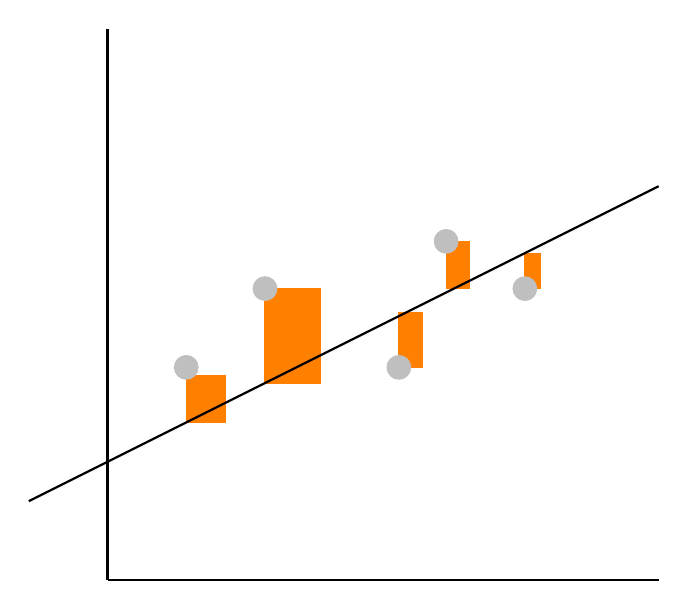
\begin{tikzpicture}
		\draw [thick] (0,0) to (0,7); % Y
		\draw [thick] (0,0) to (7,0); % X
		\draw [orange,fill] (1,2.6) rectangle (1.5,2);
		\draw [orange,fill] (2,3.7) rectangle (2.7,2.5);
		\draw [orange,fill] (3.7,2.7) rectangle (4,3.4);
		\draw [orange,fill] (4.3,4.3) rectangle (4.6,3.7);
		\draw [orange,fill] (5.3,3.7) rectangle (5.5, 4.15);		
		\draw [thick] (-1,1) to (7,5);
		\draw [lightgray,fill] (1,2.7) circle [radius=0.15];
		\draw [lightgray,fill] (2,3.7) circle [radius=0.15];
		\draw [lightgray,fill] (3.7,2.7) circle [radius=0.15];
		\draw [lightgray,fill] (4.3,4.3) circle [radius=0.15];
		\draw [lightgray,fill] (5.3,3.7) circle [radius=0.15];
		\end{tikzpicture}
	\end{center}
\end{figure}
\pagebreak
\subsubsection{R2 score}
Simple model
\begin{figure}[h!]
	\begin{center}
		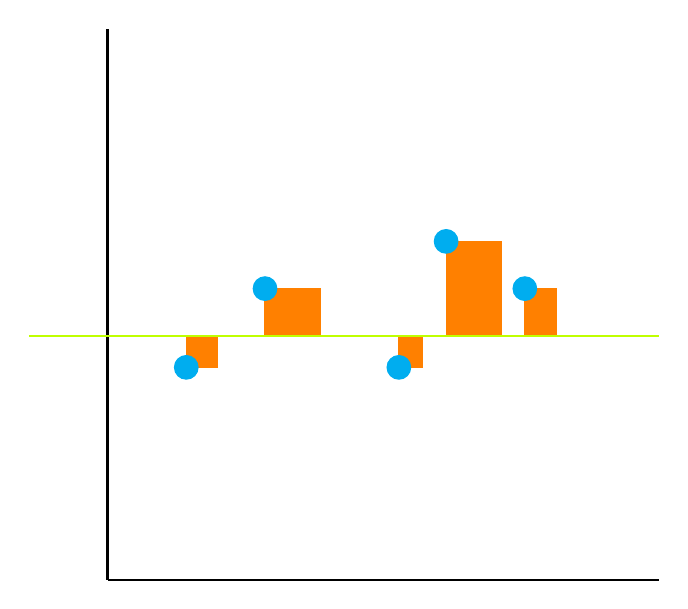
\begin{tikzpicture}
		\draw [thick] (0,0) to (0,7); % Y
		\draw [thick] (0,0) to (7,0); % X
		\draw [orange,fill] (1,2.7) rectangle (1.4,3.1);
		\draw [orange,fill] (2,3.7) rectangle (2.7,3.1);
		\draw [orange,fill] (3.7,2.7) rectangle (4,3.1);
		\draw [orange,fill] (4.3,4.3) rectangle (5,3.1);
		\draw [orange,fill] (5.3,3.7) rectangle (5.7, 3.1);
		\draw [thick,lime] (-1,3.1) to (7,3.1);
		
		\draw [cyan,fill] (1,2.7) circle [radius=0.15];
		\draw [cyan,fill] (2,3.7) circle [radius=0.15];
		\draw [cyan,fill] (3.7,2.7) circle [radius=0.15];
		\draw [cyan,fill] (4.3,4.3) circle [radius=0.15];
		\draw [cyan,fill] (5.3,3.7) circle [radius=0.15];

		\end{tikzpicture}
	\end{center}
\end{figure}
\[ R2= 1 - \frac{mean\ squared\ error\ for\ the\ linear\ regression}{mean\ squared\ error\ from\ the\ simple\ model} \]
\paragraph{Bad model} the errors should be similar R2 score should be close to 0
\paragraph{Good model} the mean squared error for the linear regression model should be a lot smaller than the mean squared error for the simple model. R2 score should be close to 1

\section{Errors}
\subsection{Underfitting (High bias)}
\paragraph{}Oversimplify the problem. The model is to simple to capture the complexity of the data
\begin{itemize}
	\item[$-$] Bad on training set
	\item[$-$] Bad on testing set
	\item[$-$] Error due to bias
\end{itemize}
\subsection{Overfitting (High variance)}
\paragraph{}Overcomplicate the problem.
\begin{itemize}
	\item[$-$] Good on training set
	\item[$-$] Bad on testing set
	\item[$-$] Error due to bias
	\item[$-$] It memorize the data instead of learn the characteristics
	\item[$-$] Error due to variance
\end{itemize}

\subsection{Cross validation}
\paragraph{} A cross validation dataset is used to check the if a model is underfitting or overfitting. Once we find a good model, we can do the final test in the testing dataset. 

NEVER use the testing dataset to check the model complexity

\paragraph{K-fold cross validation} 

\paragraph{} When training a model we split our data set in traning and testing set. However, this simple split can make us lose some important data to train our model. K-fold cross validation can help on that. 

We split the data in K buckets and train the model K times. Each time using a different bucket as the testing set and the rest of the data as the training set. In the end we calculate the avarege of the results to get the final model

\subsection{Learning curves}


\begin{figure}[ht!]
	\centering
		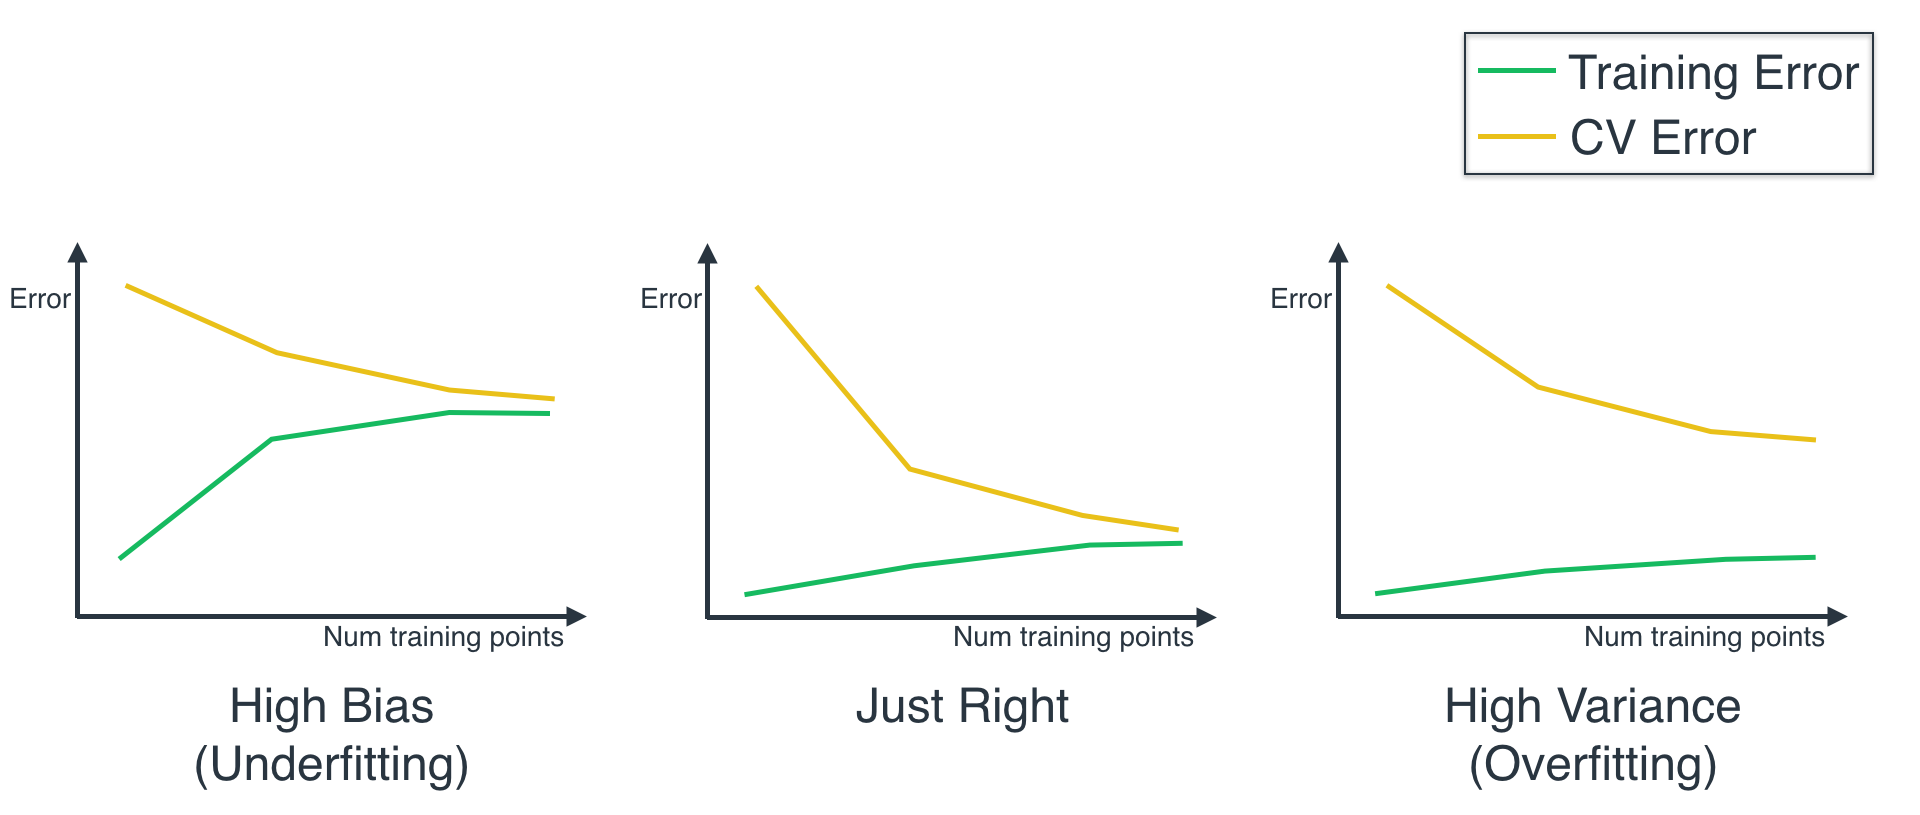
\includegraphics[width=15cm]{image/learning_curves.png}
		\caption{Learning curves of underfitting, just right and overfitting models.}
\end{figure}

\subsection{Grid search}

\paragraph{} Grid search is a hyper-parameter optimisation technique. Where a learning algorithm is trained with different parameters values and check their performance then choose the best one
\end{document}
